\subsubsection{Mixtures of Gaussians}
 \label{subsection:mog}

Mixtures of Gaussians (MoG), or the Gaussian Mixture Model (GMM), is a method of clustering (see section \ref{subsection:clustering}) that is based not on distance \ref{subsubsection:kmeans} but distribution. This method of clustering was popularized by Duda and Hart in their text \emph{Pattern Classification and Scene Analysis} \cite{mog_seminal}. This method is more effective than distance based methods because it considers the covariance of the data. Note that for K-Means clustering the distributions were spherical, but if the true clusters were more elliptical then K-Means would fail to cluster them properly. Figure \ref{fig:cluster_shapes} compares what these cluster shapes might look like and the arrows indicate the location, the arrows indicate data points that are ambiguous.

\begin{figure}[h]
	\centering
	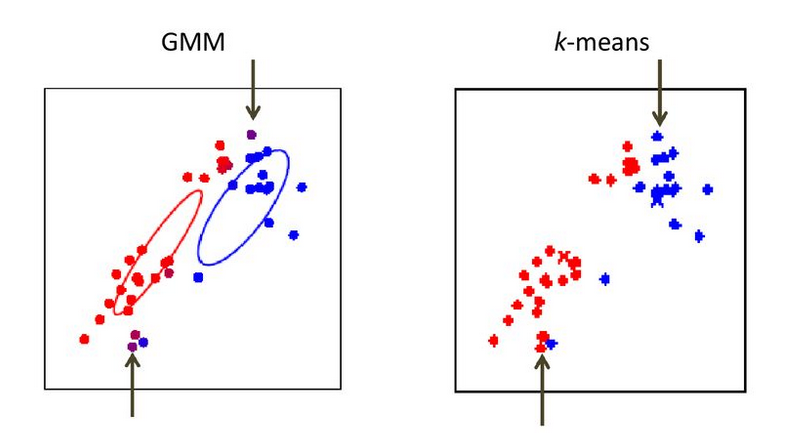
\includegraphics[width = 0.9\textwidth]{litreview/computervision/mog/mog_vs_kmeans.png}
	\captionsetup{format = hang}
	\caption{Comparison of K-Means cluster shape to GMM cluster shape. Img: Hongning Wang, University of Virginia }
	\label{fig:cluster_shapes}
\end{figure}
	
The basis of the Gaussian Mixture Model is of course the Gaussian Distribution function \ref{section:gaussian}. It is useful for probabilistic clustering because, as the Central Limit Theorem States, the distribution of the average value of the subsets of any data set will approximately converge to a Normal distribution as the number of terms in the subsets increases \cite{patterns_machine_learning}. The Mixture of Gaussian for the random variable $\boldsymbol{x}$ is achieved by super-positioning the distributions of random variable for each cluster. Equation \ref{eq:mog} describes the super-positioning of $K$ distributions for random variable $\boldsymbol{x}$, the resulting curve models the distribution of the random variable. 

\begin{equation}
p(\boldsymbol{x}) = \sum^{K}_{k = 1}\pi_k \mathcal{N}(\boldsymbol{x}|\boldsymbol{\mu_k}, \boldsymbol{\Sigma_k})
\label{eq:mog}
\end{equation}

The variable $\pi_k$ is known as the \emph{mixing coefficient} of a Gaussian distribution which controls the weighting of a particular distribution in the mixture. The sum of the mixing ratios is 1 because the complete mixture distribution represent the probability of a sample belonging to any one cluster and it must belong to one, hence

\[\sum_{k=1}^K\pi_k = 1\]

To help to understand how equation \ref{eq:mog} came about consider the random variable $\boldsymbol{z}$ of dimension K which is a binary random variable, meaning it can only have value 1 or 0. Only one element of $\boldsymbol{z}$ can be equal to 1 and all others must be 0, thus

\[\sum_{k=1}^Kz_k = 1\]

Hence there are K possible combinations of the vector $\boldsymbol{z}$. The marginal distribution over $\boldsymbol{z}$ is defined in terms of the mixing coefficients, 

\[p(z_k = 1) = \pi_k\]

That is to say the probability of $z_k$ = 1 is equal to the mixing coefficient of Gaussian distribution k. This can also be written

\[p(\boldsymbol{z}) = \prod^K_{k=1}\pi^{z_k}_k\]

The significance of $\boldsymbol{z}$ represents the assignment of a sample to a cluster which is why only one of its elements can be 1. To observe the Gaussian distribution of $\boldsymbol{z}$ in cluster $K$ we set $z_k = 1$ as described by the condition distribution,

\[p(\bm{x}|\boldsymbol{z}) = \mathcal{N}(\boldsymbol{x}|\boldsymbol{\mu_k}, \boldsymbol{\Sigma_k}) \]

Finally we can define the marginal distribution of $\boldsymbol{x}$, formerly described by \ref{eq:mog}, using the marginal distribution $p(\boldsymbol{z})$ and the conditional distribution $p(\bm{x}|\bm{z})$ as described by equation \ref{eq:mog_derive}. Figure \ref{fig:mog_compare} shows the super-positioning of individual Gaussian distributions to form a mixture of Gaussian for a one-dimensional dataset.

\begin{align}
	p(\bm{x}) 	&= p(\bm{z})p(\bm{x}|\bm{z})\\
				&= \sum^{K}_{k = 1}\pi_k \mathcal{N}(\boldsymbol{x}|\boldsymbol{\mu_k}, \boldsymbol{\Sigma_k})
\label{eq:mog_derive}
\end{align}


\begin{figure}[htbp]
    \centering
     \begin{subfigure}[b]{0.45\textwidth}
        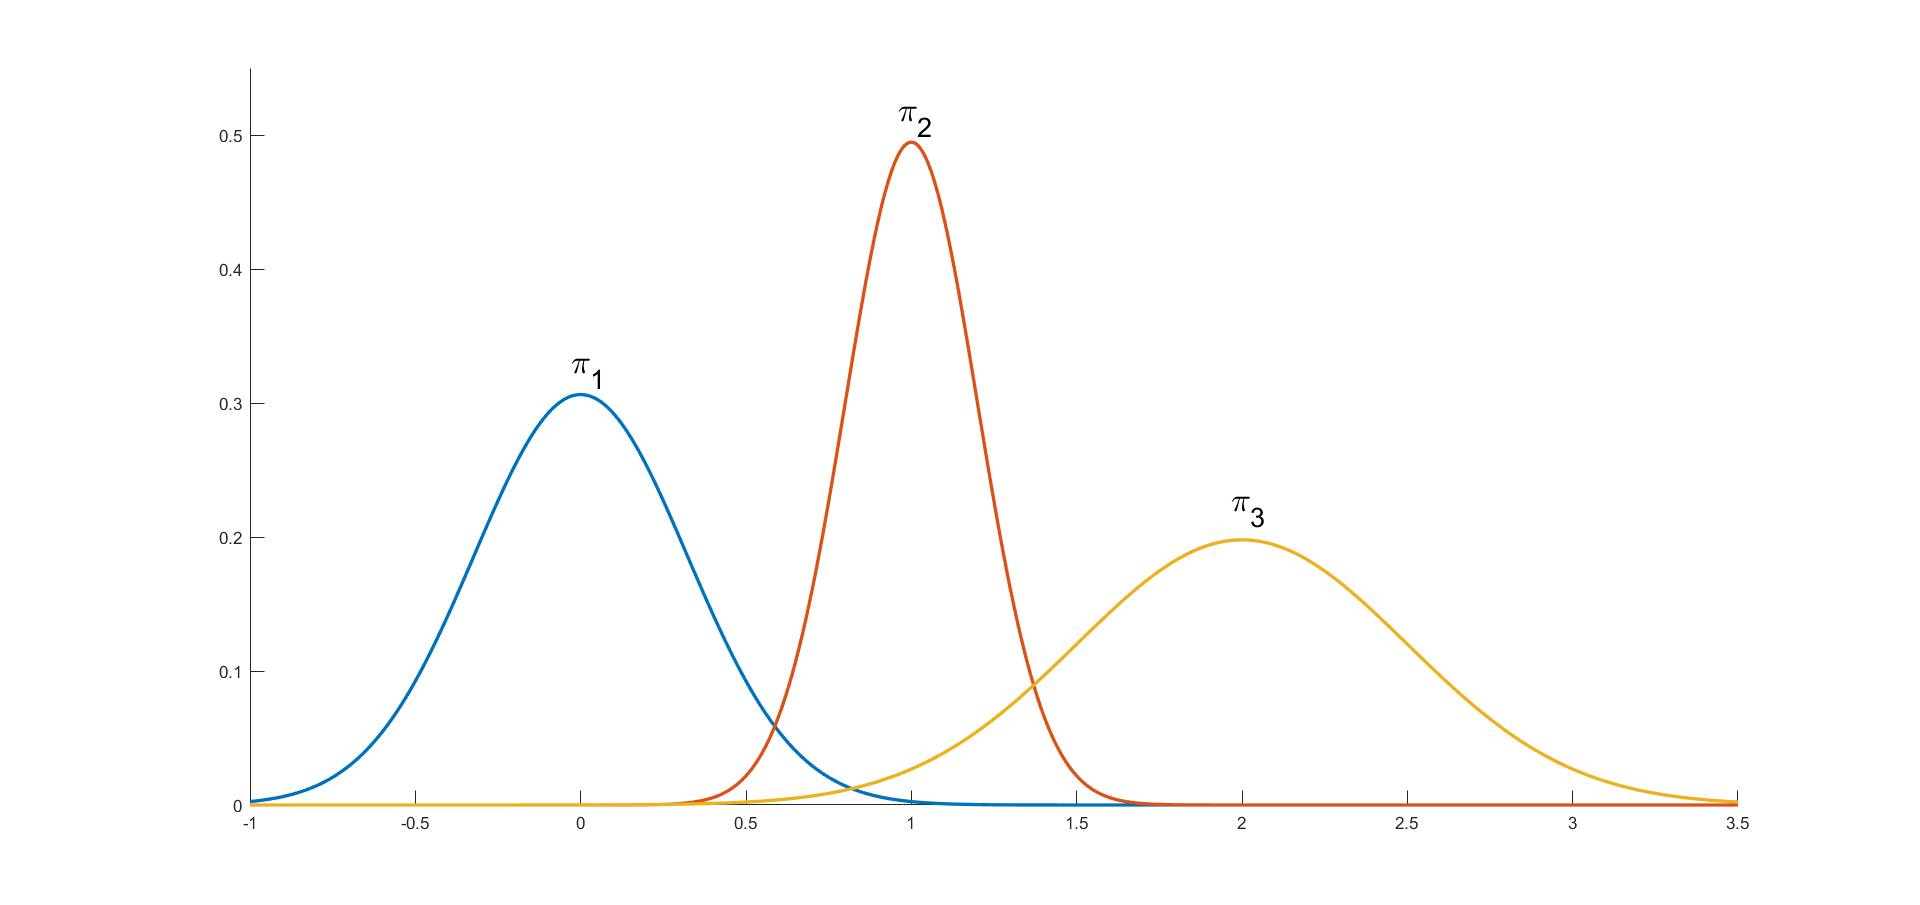
\includegraphics[width=\textwidth]{litreview/machinelearning/clustering/mog/individual_gauss.png}
	\captionsetup{format = hang}
        \caption{Three individual cluster distributions.}
        \label{fig:mog_singles}
    \end{subfigure} 
    \begin{subfigure}[b]{0.45\textwidth}
        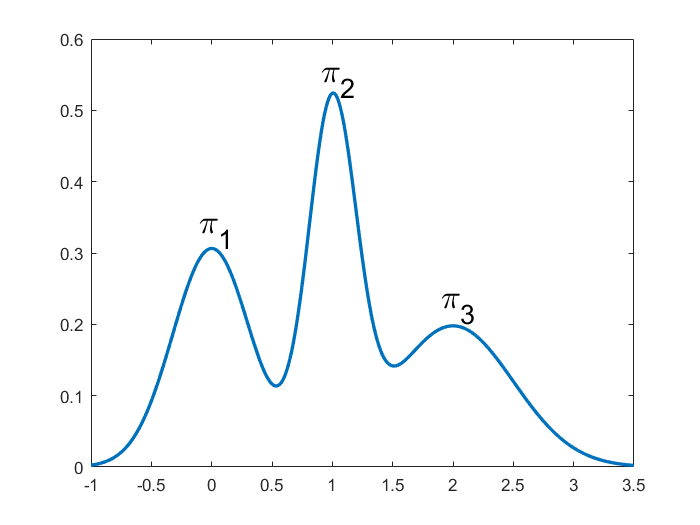
\includegraphics[width=\textwidth]{litreview/machinelearning/clustering/mog/combined_mog.png}	
	\captionsetup{format = hang}
        \caption{Super-positioned Gaussian distributions}
        \label{fig:mog_combined}
    \end{subfigure}
    \captionsetup{format = hang}
    \caption{Visualization of a Mixture of Gaussians for 1D dataset.}
    \label{fig:mog_compare}
\end{figure}

\textbf{Expectation Maximization}

Initially, cluster distributions of the GMM have random parameters but the ultimate objective of the model is to represent the cluster distribution for a given dataset. Expectation Maximization \cite{dempster_EM}\cite{emalgo} is the algorithm that determines how to update each Gaussian's parameters in a GMM. It seeks to maximize each sample's likelihood in each cluster distribution by maximizing the log likelihood function of the GMM. The log likelihood function for a GMM is the log of the GMM's likelihood function (\ref{eq:mog}) summed for each data sample and is described by equation \ref{eq:log_likelihood} where N is the number of data samples. Taking the natural log of the likelihood function simplifies the calculation as it removes the necessity to deal with exponential functions but because the natural log is monotonic the maximum value of $ln(f(x))$ is also the maximum value of $f(x)$ \cite{patterns_machine_learning}. 

\begin{equation}
\label{eq:log_likelihood}
ln p(\bm{X}|\bm{\pi},\bm{\mu},\bm{\Sigma}) = \sum_{n=1}^N ln \bigg \{ \sum^K_{k=1} \pi_k \mathcal{N}(x|\bm{\mu}_k, \bm{\Sigma}_k) \bigg \}
\end{equation}

Expectation maximization (EM) creates a probability for each sample for each cluster hence it's a soft-assignment because each sample belongs a certain amount to each cluster. Each samples cluster probability is determined according the conditional probability of $\bm{z}$ given the dataset $\bm{x}$. This probability can be thought of as the responsibility of cluster $k$ for describing dataset $\bm{x}$ and is denoted, $\gamma(z_k)$. This probability is derived according to Bayes Theorem (appendix \ref{section:bayes}) and described by equation \ref{eq:bayes_em}.

\begin{align}
    \label{eq:bayes_em}
    \gamma(z_k) \equiv p(z_k = 1|\bm{x}) &= \frac{p(z_k=1)p(\bm{x}|z_k=1)}{\sum\limits_{j=1}^{K}p(z_j=1)p(\bm{x}|z_j=1)}\\
                                     &= \frac{\pi_k \mathcal{N}(\bm{x}|\bm{\mu_k},\bm{\Sigma_k})}{\sum\limits_{j=1}^{K}\pi_j\mathcal{N}(\bm{x}|\bm{\mu_j},\bm{\Sigma_j})}
\end{align}

To find the parameters for a Gaussian, $k$, that generate the maximum likelihood for a data sample, $\bm{x_n}$, we take the derivative of the log likelihood \ref{eq:log_likelihood} in terms of the mean, $\bm{\mu_k}$, and covariance, $\bm{\sigma_k}$ and set it's value to zero. Equation \ref{eq:derivative_mean} shows the derivative of the log likelihood taken in terms of the mean, $\bm{\mu_k}$ \cite{patterns_machine_learning}. Note that $\gamma(z_nk)$ is the responsibility of cluster $k$ for sample $x_n$.

\begin{align}
    0   &= -\sum^N_{n=1}\frac{\pi_k \mathcal{N}(\bm{x_n}|\bm{\mu_k},\bm{\Sigma_k})}{\sum\limits_{j=1}^{K}\pi_j\mathcal{N}(\bm{x}|\bm{\mu_j},        \bm{\Sigma_j})}\bm{\Sigma_k}(\bm{x_n} - \bm{\mu_k})\\
        &= -\sum^N_{n=1}\gamma(z_{nk})\bm{\Sigma_k}(\bm{x_n} - \bm{\mu_k})
    \label{eq:derivative_mean}
\end{align}

This can be rearranged to give the value of the updated mean, $\bm{\mu_k}$ for cluster distribution $k$, where $N$ is the number of samples in $\bm{x}$ 

\begin{equation}
    \label{eq:updated_mean}
    \bm{\mu_k} = \frac{1}{N_k}\sum_{n=1}^N \gamma(z_nk)\bm{x_n}
\end{equation}

where 

\begin{equation}
    \label{eq:nk}
    N_k = \sum_{n=1}^N \gamma(z_nk)
\end{equation}

Therefore we can think of the updated mean as simply the average of the cluster samples weighted by the responsibility of each cluster to each sample. The updated covariance matrix $\bm{Sigma_k}$ is evaluated similarly, by taking the derivative of the log likelihood in terms of covariance and setting it equal to zero, which yields the result

\begin{equation}
    \label{eq:updated_covariance}
    \bm{Sigma_k} = \frac{1}{N_k}\sum_{n=1}^{N}\gamma(z_{nk})(\bm{x_n}-\bm{\mu_k})(\bm{x_n}-\bm{\mu_k})^T 
\end{equation}

The updated and maximized mixing coefficient of the cluster distributions $\pi_k$ is calculated as 

\begin{equation}
    \label{eq:updated_mixing_coefficient}
    \pi_k = \frac{N_k}{N}
\end{equation}

The process of expectation maximization for a GMM is outlined by algorithm \ref{algorithm:em}.


\begin{algorithm}
    \SetAlgoLined
    \KwInput{Set of data vectors X of size M} 
    \KwOutput{K sets of clustered data vectors}
    Initialize the desired number of clusters $K$\;
    Initialise a list of $K$ random cluster centroids $\mu$\;
    \While{$\mu$ elements have not converged}{
        \For{i = 0 to M}
        {
            distOld = $\inf$
            \For{j = 0 to K}{
                distnew = EuclideanDistance(X[i], $\mu[j]$)\;
                \If{distNew $<$ distOld}{
                    distOld = distNew\;
                    $\mu_j$.append(X[i])\;
                }
            }
        }
        \For{p = 0 to K}{
            centroidList.append(average($\mu[p]$))\;
        }
    }
    \caption{K Means Clustering \cite{oreilly_python}}
    \label{algorithm:em}
\end{algorithm}















A binary indicator $z_{i}$ exists for every sample $x_i$, it is 1 if the sample belongs in the cluster $k$ and 0 otherwise such that $z_{ik} \in \{0, 1\}$ and $\sum_k z_{ik} = 1$. If the data is multidimensional then the sample and indicator are both vectors, $\bm{x}$ and $\bm{z}$. The marginal probability $p(\bm{z}_{k} = 1)$ is the probability that a sample $\bm{x}$ is in cluster $k$. This quantity is completely specified by the mixture weight $\pi_k$ for each Gaussian because the area under a Gaussian component is equal to its mixing ratio, i.e.

\begin{equation}
	\label{eq:marginalk}
	p(\bm{z}_{k}=1) = \pi_k 
\end{equation}
	
If we know that a sample $\bm{x}$ is from cluster $k$ the \emph{likelihood} of seeing it in the associated Gaussian is the value of the Gaussian at that point,
\begin{equation}
	\label{eq:cond}
	p(\bm{x}\, |\, \bm{z}_{k} = 1) = \mathcal{N}(\bm{x}\, |\,\bm{\mu_k}, \bm{\Sigma_k})
\end{equation}

The conditional probability of $\bm{z}_{ik}$ given the value of sample, $\bm{x}_i$ is denoted as $\gamma(\bm{z}_{ik})$. This is the probability that a sample belongs to cluster $k$ given its value $\bm{x}_i$ and is the quantity of interest when trying to classify a sample.  Using Bayes Theorem [REF APPENDIX] quantity can be found 

\begin{align}
	\gamma(\bm{z}_{ik}) \equiv p(\bm{z}_{ik} =1 | \bm{x}_i)
	\label{eq:gamma2}
	&= \frac{p(\bm{z}_{ik}=1)p(\bm{x}_i\, |\, \bm{z}_{ik} = 1)}{\sum^K_{j=1}p(\bm{z}_{jk}=1)p(\bm{x}_j\, |\, \bm{z}_{jk} = 1)}\\ 
	\label{eq:gamma3}
	&= \frac{\pi_k\, \mathcal{N}(\bm{x}\,|\,\bm{\mu_k},\bm{\Sigma_k})}{\sum_{j=1}^{K}\pi_k\, \mathcal{N}(\bm{x}\,|\,\bm{\mu_k},\bm{\Sigma_k})}
\end{align}


To maximize the likelihood of each sample being in each Gaussian the distribution parameters are modified. This is achieved by taking derivatives of the log of the likelihood function (\ref{eq:likelihood}) with respect to each Gaussian parameter and setting the result to 0 to find local maxima. To take the log of the likelihood function assume all samples in are in an $N \times D$ matrix $\bm{X}$ and the corresponding indicators are in an $ N \times K$ matrix $\bm{Z}$. 

\begin{equation}
\label{eq:log}
ln\,p(X|\bm{\pi}, \bm{\mu}, \bm{\Sigma}) = \sum_{n=1}^N
ln \Bigg\{ \sum_{k=1}^K \pi_k\mathcal(N)(\bm{x}_n|\bm{\mu}_k,\bm{\Sigma}_k)\Bigg\}
\end{equation}







\centerline{}

The EM algorithm is comprised of [X] steps

%% EM STEPS %%
\begin{enumerate}
	\item Generate the initial K Gaussian parameters mean $\bm{\mu}_{k}$, covariance $\bm{\Sigma}_k$ and mixing ratios $\pi_k$ either randomly or informed by a histogram.
	\item Estimate the likelihood sample n was generated by cluster k for all samples. 
	\begin{equation}
		\gamma(\bm{z}_{ik})=\frac{\pi_k\, \mathcal{N}(\bm{x}\,|\,\bm{\mu_k},\bm{\Sigma_k})}{\sum_{j=1}^{K}\pi_k\, \mathcal{N}(\bm{x}\,|\,\bm{\mu_k},\bm{\Sigma_k})}
	\end{equation}

	\item Maximize the Gaussian parameter using derivatives of log likelihood for each parameter.
	\begin{align}	
	\label{eq:mean}
	\bm{\mu}_{k}^{new} &= \frac{1}{N_k}\sum_{n=1}^N \gamma(z_{nk} ) \bm{x}_n \\
	\label{eq:covariance}
	\bm{\Sigma}_k^{new} &=  \frac{1}{N_k}\sum_{n=1}^N\gamma(z_{nk})(\bm{x}_n- \bm{\mu}_k^{new})(\bm{x}_n - \bm{\mu}_k^{new})^T \\
	\label{eq:ratio}
	\pi_k &= \frac{N_k}{N}
	\end{align}
	where \newline
	\[N_k = \sum_{i} z_{ik}\]
	\item Repeat steps 2 and 3 until convergence of log likelihood (\ref{eq:likelihood}) or parameters. 
\end{enumerate}

The Gaussian Mixture Model method of clustering is computationally complex compared to K-Means however it's ability to differentiate ambiguous samples by considering covariance is superior. 


